%This is a very basic  BE PROJECT PRELIMINARY template.

%############################################# 
%#########Author :  PROJECT###########
%#########COMPUTER ENGINEERING############


\documentclass[oneside,a4paper,12pt]{report}
\usepackage{titlesec}
\titleformat{\chapter}[display]
  {\normalfont\huge\bfseries\raggedright}
  {\chaptertitlename\ \thechapter}
  {20pt}
  {\Huge}

\usepackage[a4paper,left=1.15in,right=0.95in,top=0.95in,bottom=0.95in]{geometry}
\usepackage{amsmath}
\usepackage{etoolbox}
\usepackage{needspace}
\usepackage{tocloft}
\usepackage{titlesec}
\usepackage{graphicx}
\usepackage{fancyhdr}
\usepackage{float}
\usepackage{appendix}
\usepackage{booktabs}
\usepackage{tabularx}
\usepackage{array}
\usepackage{multirow}
\usepackage{xcolor}
\usepackage{listings}
\usepackage{caption}
\usepackage{setspace}
\usepackage[ruled,vlined,linesnumbered]{algorithm2e}
\usepackage[nottoc,notlot,notlof]{tocbibind}
\usepackage{cite}
\usepackage[hidelinks]{hyperref}

\graphicspath{{figures/}}
\setcounter{secnumdepth}{3}
\setcounter{tocdepth}{1}
\setstretch{1.0}
\emergencystretch=2em
\captionsetup{font=small,labelfont=bf,skip=4pt}
\setlength{\parindent}{0mm}
\setlength{\parskip}{5pt}
\raggedbottom
\renewcommand{\arraystretch}{1.2}

\definecolor{codebg}{RGB}{246,248,247}
\definecolor{codeink}{RGB}{27,31,29}
\definecolor{codecom}{RGB}{31,122,90}
\lstset{
  basicstyle=\ttfamily\footnotesize\color{codeink},
  backgroundcolor=\color{codebg},
  commentstyle=\color{codecom},
  frame=single, rulecolor=\color{black!20},
  breaklines=true, columns=fullflexible, keepspaces=true,
  xleftmargin=2pt, xrightmargin=2pt, aboveskip=6pt, belowskip=6pt
}

\pagestyle{fancy}
\fancyhf{}
\renewcommand{\headrulewidth}{0pt}
\cfoot{\thepage}
\fancypagestyle{plain}{\fancyhf{}\renewcommand{\headrulewidth}{0pt}\cfoot{\thepage}}

% =====================================================================
%  EDIT THIS BLOCK ONLY. Every name on the cover, certificate, approval
%  sheet and acknowledgement comes from here. Items in [brackets] are
%  placeholders that must be replaced before submission.
% =====================================================================
\newcommand{\TitleLineA}{Model Compression Toolkit:}
\newcommand{\TitleLineB}{A Unified Platform for Pruning, Quantization}
\newcommand{\TitleLineC}{and Knowledge Distillation}
\newcommand{\ProjectTitle}{\TitleLineA{} \TitleLineB{} \TitleLineC}
\newcommand{\ProjectTitleBlock}{\TitleLineA\\[2pt] \TitleLineB\\[2pt] \TitleLineC}
\newcommand{\StudentA}{Relan Pratiksha Virendra}
\newcommand{\ExamA}{23054491246054}
\newcommand{\StudentB}{Joshi Bhagyesh Pradeep}
\newcommand{\ExamB}{23054491245053}
\newcommand{\StudentC}{Vora Avinash Ritesh}
\newcommand{\ExamC}{24054491245504}
\newcommand{\StudentD}{Joshi Yesha Pratik}
\newcommand{\ExamD}{24054491245512}
\newcommand{\Guide}{Dr. Kavita Patil}
\newcommand{\Hod}{Dr. Makrand Shahade}
\newcommand{\Principal}{Dr. Nilesh Salunke}
\newcommand{\Coordinator}{Dr. Kavita Patil}
\newcommand{\AcademicYear}{2026--2027}
\newcommand{\Semester}{VII}
% =====================================================================

\makeatletter
\makeatother
\setlength{\cftbeforechapskip}{3pt}
\setlength{\cftbeforetoctitleskip}{0pt}\setlength{\cftaftertoctitleskip}{18pt}
\setlength{\cftbeforeloftitleskip}{0pt}\setlength{\cftafterloftitleskip}{18pt}
\setlength{\cftbeforelottitleskip}{0pt}\setlength{\cftafterlottitleskip}{18pt}
\setlength{\cftbeforesecskip}{0pt}
\setlength{\cftbeforefigskip}{0pt}
\setlength{\cftbeforetabskip}{0pt}
\renewcommand{\cftchapfont}{\bfseries\small}
\renewcommand{\cftsecfont}{\small}
\renewcommand{\cftfigfont}{\small}
\renewcommand{\cfttabfont}{\small}
\titlespacing*{\chapter}{0pt}{-10pt}{14pt}
\titleformat{\section}{\bfseries\large}{\thesection}{0.6em}{}
\titlespacing*{\section}{0pt}{12pt}{4pt}
\titleformat{\subsection}{\bfseries\normalsize}{\thesubsection}{0.6em}{}
\titlespacing*{\subsection}{0pt}{9pt}{3pt}
\newcommand{\code}[1]{\texttt{\small #1}}

\begin{document}
\pagenumbering{gobble}

% ------------------------------------------------------------ cover, certificate, approval sheet
% These three pages use symmetric margins so that everything is centred on the page.
\newgeometry{left=1in,right=1in,top=1in,bottom=1in}
\newcommand{\NameBlock}{%
  \begin{tabular}{@{}l@{\hspace{1.5cm}}l@{}}
    \StudentA & Exam No: \ExamA\\[2pt]
    \StudentB & Exam No: \ExamB\\[2pt]
    \StudentC & Exam No: \ExamC\\[2pt]
    \StudentD & Exam No: \ExamD
  \end{tabular}}
\newcommand{\SignBlock}[3]{\parbox[t]{0.46\textwidth}{\centering\textbf{#1}\\ #2\\ #3}}

% ---- cover
\thispagestyle{empty}
\begin{center}
{\bfseries\large A PROJECT PHASE-I REPORT ON}\par
\vfill
{\bfseries\fontsize{20}{26}\selectfont \ProjectTitleBlock\par}
\vfill
SUBMITTED TOWARDS THE PARTIAL FULFILLMENT OF\\ THE ACADEMIC REQUIREMENTS FOR THE SEMESTER \Semester\par
\vspace{0.5cm}
{\bfseries\Large BACHELOR OF TECHNOLOGY}\par
\vspace{0.15cm}
{\bfseries\large (Computer Engineering)}\par
\vfill
{\bfseries\large Submitted by}\par
\vspace{0.35cm}
\NameBlock\par
\vfill
{\bfseries\large Under the Guidance of}\par
\vspace{0.25cm}
{\bfseries\Large \Guide}\par
\vfill

\includegraphics[width=95pt]{Update_logo_SVKM.jpg}\par
\vspace{0.5cm}
{\bfseries\large SHRI VILE PARLE KELAVANI MANDAL'S\\ INSTITUTE OF TECHNOLOGY, DHULE 424001}\par
\vspace{0.3cm}
Affiliated to\par
\vspace{0.1cm}
{\bfseries DR.\ BABASAHEB AMBEDKAR\\ TECHNOLOGICAL UNIVERSITY, LONERE}\par
\vspace{0.3cm}
{\bfseries Year: \AcademicYear}\par
\end{center}
\newpage

% ---- certificate
\thispagestyle{empty}
\begin{center}

\includegraphics[width=90pt]{Update_logo_SVKM.jpg}\par
\vspace{0.8cm}
{\bfseries\fontsize{22}{26}\selectfont CERTIFICATE}\par
\vfill
This is to certify that the project entitled\par
\vspace{0.4cm}
{\bfseries\Large \ProjectTitleBlock\par}
\vspace{0.4cm}
Submitted by\par
\vspace{0.3cm}
\NameBlock\par
\end{center}
\vspace{0.2cm}
{\setstretch{1.3}\hyphenpenalty=10000\noindent is a bonafide work carried out by the students under the supervision of \textbf{\mbox{\Guide}} and it is submitted towards the partial fulfillment of the academic requirements for Semester \Semester{} (Computer Engineering) of Dr.\ Babasaheb Ambedkar Technological University, Lonere.\par}
\vfill
\vfill
\noindent\SignBlock{\Guide}{Internal Guide}{Dept.\ of Computer Engineering}\hfill\SignBlock{\Hod}{Head of Department}{Dept.\ of Computer Engineering}
\vfill
\vfill
\begin{center}
\textbf{\Principal}\\ Principal\\ SVKM's Institute of Technology, Dhule
\end{center}
\vfill
\vfill
\noindent Signature of Internal Examiner \hfill Signature of External Examiner\par
\newpage

% ---- approval sheet
\thispagestyle{empty}
\begin{center}
\vspace*{0.3cm}
{\bfseries\fontsize{22}{26}\selectfont PROJECT APPROVAL SHEET}\par
\vfill
A Project Title\par
\vspace{0.6cm}
{\bfseries\Large \ProjectTitleBlock\par}
\vspace{0.8cm}
is successfully completed by\par
\vspace{0.6cm}
\NameBlock\par
\vspace{0.8cm}
at\par
\vspace{0.8cm}
{\bfseries\large DEPARTMENT OF COMPUTER ENGINEERING}\par
\vspace{0.5cm}
SHRI VILE PARLE KELAVANI MANDAL'S\\ INSTITUTE OF TECHNOLOGY, DHULE\par
\vspace{0.5cm}
DR.\ BABASAHEB AMBEDKAR\\ TECHNOLOGICAL UNIVERSITY, LONERE\par
\vspace{0.8cm}
ACADEMIC YEAR \AcademicYear\par
\end{center}
\vfill
\noindent\SignBlock{\Guide}{Internal Guide}{Dept.\ of Computer Engineering}\hfill\SignBlock{\Coordinator}{Project Coordinator}{Dept.\ of Computer Engineering}
\vspace*{0.8cm}
\newpage
\restoregeometry

\pagenumbering{roman}

% ------------------------------------------------------------ acknowledgement
\begin{center}{\bfseries\Large Acknowledgements}\end{center}
\vspace{0.6cm}
It gives us great pleasure to present the final-year project report on \textbf{``\ProjectTitle''}.

We would like to thank our internal project guide, \textbf{\Guide}, for the guidance, patience and critical feedback that shaped this work. The repeated insistence that every claim in the project be backed by a measurement is the reason this report separates what was measured from what was only expected.

We are grateful to \textbf{\Hod}, Head of the Department of Computer Engineering, for his support and suggestions, and to the Principal, \textbf{\Principal}, for the infrastructure, encouragement and support provided to us.

We also thank all teaching and non-teaching staff of the Department of Computer Engineering, and our friends, who helped us directly or indirectly in completing this work. We acknowledge the authors of the open-source libraries on which the toolkit is built, namely PyTorch, Torch-Pruning, ONNX and ONNX Runtime, and the free GPU time provided by Kaggle that made the larger experiments possible.

\vspace{1.6cm}
\hfill\begin{tabular}{@{}l@{}}
\StudentA\\ \StudentB\\ \StudentC\\ \StudentD\\ (B.Tech Computer Engineering)
\end{tabular}
\newpage

{  \newpage {\bfseries \fontsize{14}{12} \selectfont \centerline{Abstract} 
\vspace*{2\baselineskip}} \setlength{\parindent}{11mm} }
{ \setlength{\parindent}{0mm} }
Convolutional Neural Networks (CNN) prove to be highly accurate for image classification and tasks relating to computer vision but their computational and storage requirements stand an obstacle for their deployment on devices which are resource constrained. Model compression techniques such as pruning, quantization and knowledge distillation are used to extensively reduce the model complexity while preserving the predictive performance, but the compression is traditionally evaluated and reported through proxy methods of floating point operation counts(FLOPs), parameter counts, or on disk model file size. These measures do not always translate into equivalent reductions in the actual inference latency on a CPU.
The proposed system presents a staged compression toolkit in which every reported quantity is measured upon the deployment runtime  rather than inferring it from a model structure. is a model compression toolkit for convolutional neural networks for applying and evaluating multiple compression techniques using a common measurement protocol, that integrates structured channel pruning, batch normalization re-estimation, logit based knowledge distillation and quantization within a dependency aware pipeline.  The stages organized as a sequential pipeline where we can measure the contribution of every stage independently. In contrast to the previous approaches, in the proposed system every stage of the pipeline is evaluated using wall-clock latency inference latency directly on the target CPU rather than estimation from FLOPs or parameter counts, while considering the model accuracy, on-disk model size, parameter count, latency distribution and layer level sensitivity.
From the survey of twenty papers spanning pruning, quantization, distillation reveals that a large proportion of approaches use FLOPs, parameter counts or model size as their only metrics to measure compression and none use CPU latency against a named instruction-set architecture establishing a measurement gap that this work addresses directly. The proposed system further introduces a translation efficiency metric, quantifying the fraction of a claimed proxy-based reduction survives translation into real latency, and a per-stage attribution protocol that isolates the accuracy recovered by batch-norm re-estimation alone, before any gradient-based fine-tuning. As this recovery step is absent in the prior sequential pipeline, the proposed system is hypothesized to retain the baseline accuracy at a matched pruning ratio. This paper presents the design rationale, mathematical formulation, system architecture, and experimental protocol for a full factorial evaluation across pruning ratios and precisions on CIFAR-10, along with the toolkit's expected outcomes.



\vspace{0.4cm}
\textbf{Keywords:} Model compression, structured pruning,  knowledge distillation, quantization, CPU latency, wall-clock latency.






\newpage
 \tableofcontents
 \newpage
 \listoffigures
 \newpage
 \listoftables


\chapter{Synopsis}

\pagenumbering{arabic}
\section{Project Title}

Model Compression Toolkit (implemented as the Python package CompressKit): A Unified Platform for Pruning, Quantization and Knowledge Distillation.



\section{Domain of Project}  

Efficient Deep Learning and Model Compression, focusing on Convolutional Neural Networks (CNNs), structured pruning, knowledge distillation, post-training quantization, and performance measurement using CPU inference runtimes.


\section{Problem Statement}
The problem this work addresses is hence not the design of a new compression algorithm. The underlying algorithms dependency-graph structured pruning, temperature-scaled distillation, static integer quantization are mature and well implemented in existing libraries~\cite{wang2025,hinton2015}. The problem is the absence of a decision and verification layer: a system that determines how much of each technique a particular model on a particular host requires, that refuses to apply a transformation whose benefit the host cannot realize, and that reports what was actually achieved rather than what the model's structure implies should have been achieved~\cite{chae2026,abdelsalam2025}. Concretely, four failure modes must be eliminated. A compression stage must not be able to report a size reduction as a speed improvement. A pruning ratio requested by the user must not be silently ignored for a subset of layers. An accuracy figure must not be computed on a model artifact different from the one that will be deployed. And a per-layer decision which layers to compress hard, which to protect must be derived from measurement rather than from a uniform default applied blindly across network depth~\cite{khan2025}.

\section{Objectives and Expected Outcomes }  
The objectives of this work are as follows:
\vspace*{0.5\baselineskip}

\begin{enumerate}
\item To design a staged compression pipeline in which stage ordering is enforced structurally, so that a transformation which invalidates a later stage cannot precede it~\cite{chae2026,wang2025}.
\vspace*{0.5\baselineskip}

\item To formulate a per-layer SIMD-alignment rule that keeps pruned channel widths on vector-register boundaries without allowing a single narrow layer to force the relaxation of alignment across the entire network.
\vspace*{0.5\baselineskip}

\item To derive a label-free, backpropagation-free per-layer sensitivity measure capable of ranking layers by the output distortion their compression induces, and to use that single ranking for two distinct decisions - quantization exclusion and non-uniform pruning allocation~\cite{he2018,abdelsalam2025}.
\vspace*{0.5\baselineskip}

\item To gate the target numerical precision on a runtime probe of the host instruction set rather than on an assumption about the deployment target~\cite{chen2021,fang2026}.
\vspace*{0.5\baselineskip}

\item To define a budget-driven search that terminates at the least aggressive configuration satisfying a declared latency, accuracy and size constraint, and to specify a measurement protocol under which the reported figures are directly comparable across precisions~\cite{he2018}.
\vspace*{0.5\baselineskip}
\end{enumerate}
\newpage
\vspace{-1cm}
\chapter{Introduction}
\section{Overview of Project Domain}

Convolutional neural networks (CNNs) are the standard solution for image classification, and their accuracy comes with cost: ResNet and VGG families carry millions to hundreds of millions of parameters and tens to thousands of millions of multiply-accumulate operations per image~\cite{he2016,simonyan2015}. Deploying them on CPUs requires reducing the memory footprint of the weights and the time of one forward pass.

Three technique families dominate the literature.

\textbf{Pruning} removes structure from the network. Unstructured pruning zeroes individual weights, which leaves every tensor the same size and gives no speed-up on a standard CPU runtime. Structured pruning removes whole channels or filters, which shrinks the matrix multiplications themselves. This project uses structured pruning only.

\textbf{Quantization} lowers the numeric precision of weights and activations, typically from 32-bit float to 8-bit integer (INT8) or 16-bit float (FP16)~\cite{jacob2018}. File size falls in proportion to the bit width, but latency falls only when the processor has instructions that compute directly in the lower precision.

\textbf{Knowledge distillation} trains a smaller student against the soft output distribution of a larger teacher~\cite{hinton2015}. Decoupled KD splits the loss into a target-class and a non-target-class term that can be weighted separately~\cite{zhao2022}.

\begin{figure}[!htbp]
\centering
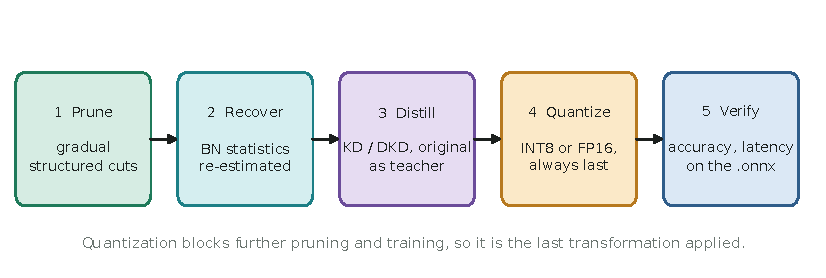
\includegraphics[width=\textwidth]{fig_pipeline.pdf}
\caption{Order of Operations in CompressKit}
\label{fig:pipeline}
\end{figure}
The purpose is to make compression a repeatable engineering step with a measurable result instead of a sequence of ad-hoc scripts. The toolkit applies to CNN image classifiers that export to ONNX, on the CPU targets where ONNX Runtime's CPU provider is used: laptops, kiosks, industrial controllers and single-board computers. Typical use is to take a model trained for a specific task, state a budget such as ``at most 0.45 ms median latency and at most 8 points of accuracy loss'', and obtain a file that meets it or a statement that it cannot.

\section{Scope of the Project}
\textbf{In scope.} Classification CNNs with convolution, batch normalisation, residual or plain stacking and a linear classifier head; structured pruning, KD and DKD, INT8 and FP16 post-training quantization, QAT as a fallback; CIFAR-10, a human-action-recognition image dataset, and any image-folder dataset; CPU measurement through ONNX Runtime; a single-notebook workflow on Kaggle and a command-line interface.

\textbf{Out of scope.} Object detection and segmentation models; transformer architectures; GPU or NPU latency; training from scratch beyond the baselines needed to have something to compress. Depthwise-separable networks (MobileNet style) were not exercised and are not claimed.

\section{Organisation of the Report}
Chapter~3 surveys eleven related papers and extracts the gaps that motivate the design. Chapter~4 gives the project plan and timeline. Chapter~5 specifies the requirements and datasets. Chapter~6 presents the proposed system: architecture, algorithms and diagrams. Chapter~7 describes the implementation and the measured results. Chapter~8 concludes and lists future work.




\chapter{Literature Survey }
\section{Related Work Done }
The increasing size and complexity of deep neural networks (DNNs) have rendered DNNs challenging to deploy on devices with limited resources, as large networks require significant amounts of memory, computational resources, energy, and inference time to perform. Therefore, research has focused on model compression techniques such as pruning, quantization, and knowledge distillation (KD) to reduce model size while maintaining prediction accuracy. These techniques underpin model compression pipelines for on-device and edge-based artificial intelligence systems.

Chae and Seo~\cite{chae2026} investigated an integrated pipeline combining pruning, quantization, and knowledge distillation. Their research highlighted the limitations of applying compression techniques on their own, since pruning, quantization, and knowledge distillation each affect the model differently. Their experiments examined different combinations of pruning and quantization. They also created compression and efficiency scores to measure both how much the model shrinks and how well it performs and hence provides performance preservation.

He et al.~\cite{he2018} introduced AMC (AutoML for Model Compression), an AutoML-based framework that uses reinforcement learning to automatically determine layer-wise pruning ratios, which eradicates the need for hand-tuned, uniform sparsity targets across network depth. This work established that a learned, layer-wise sensitivity search could surpass uniform pruning schedules, even though the search objective is formulated in terms of a proxy metric which maybe parameter count or FLOPs rather than measured latency. This approach achieved higher compression ratios with better accuracy retention than rule-based methods, and demonstrates real-world latency gains on mobile hardware, 1.8x speedup on an Android device with negligible accuracy loss.

Abdel-Salam et al.~\cite{abdelsalam2025} proposed VLCQ (Variable-Length Coding Quantization) as a data-free post- training quantization technique that uses variable-length encoding to exploit the non-uniform distribution of neural-network weights. The method does not require access to the original training dataset or model fine-tuning, making it applicable when retraining is computationally expensive, or the training dataset is unavailable. Experiments across image classification, segmentation, and object detection demonstrated up to 6x compression compared with FP32 and up to 12.25x compression with less than 4\% performance loss in selected settings.

Chen et al.~\cite{chen2021} studied the use of quantization for accurate edge computing and challenged the notion that quantization always reduces accuracy. They tested incremental quantization on biomedical image segmentation, ImageNet image classification, and automatic speech recognition. They showed that quantization can act as a form of regularization and even improve model accuracy by reducing overfitting. The experiments reported accuracy gains of 1\%, 1.95\%, and 4.23\% for the three applications, respectively, while achieving a 3.5x-6.4x memory reduction. However, the benefits of quantization depend on model size, bit-width, and hardware support, and extremely low bit-width representations can decrease accuracy; speed improvements depend on whether the underlying hardware supports the required operations.

Wang et al.~\cite{wang2025} proposed an Iterative Transfer Model Compression (ITMC) framework that combines Transfer Knowledge Distillation (TKD) and Adaptive Channel Pruning (ACP) and applies the techniques iteratively instead of as an independent post-processing step. In knowledge distillation, the teacher and student models are adapted to the target domain, where adaptive channel pruning removes redundant channels according to the training process. This approach targets to reduce model complexity while minimizing the accuracy degradation normally associated with aggressive pruning.

Khan and Rafat~\cite{khan2025} observed that conventional compression pipelines traditionally decouple pruning and quantization from training, and standard knowledge distillation relies on a full-precision teacher that is limiting its effectiveness once the student model is itself compressed. To address this, they proposed CQKD (Cluster-Quantized Knowledge Distillation), a framework that integrates structured pruning, knowledge distillation, and cluster-based weight quantization directly into a single training loop rather than treating these as separate stages. This joint formulation is reported to achieve approximately 34,000x compression while preserving accuracy, targeting deployment of CNN-based vision models on resource-constrained hardware.

Fang et al.~\cite{fang2026} investigated Quantization-Aware Training for Federated Learning (QAT-FL) to address the quantization error encountered during communication between distributed devices. Their approach inserted a fake-quantization module during training, allowing the model to adapt to the effects of quantization before deployment. Experiments on MNIST, CIFAR-10, and FEMNIST showed improvements in training loss and inference accuracy compared with post- training quantization approaches.

Xu et al.~\cite{xu2024} observed that conventional KD treats all non-target classes as an undifferentiated group, surpassing two distinct sources of knowledge that is relationships between the target class and its most similar (head) categories, and the discriminative signal carried by dissimilar (tail) categories. They proposed ReKD, which reformulates KD into two independently weighted components of Top-K Inter-class Similar Distillation (TISD) for head categories and Non-Top-K Inter-class Discriminability (NTID) for tail categories that is enabling the student to more effectively absorb both types of knowledge than uniform-weighting KD baselines.

Zhao et al.~\cite{zhao2022} decomposed the classical KD loss into target class knowledge distillation (TCKD) and non-target class knowledge distillation (NCKD), showing that NCKD which is knowledge encoded in the relationships among non-target classes which is the primary driver of KD's effectiveness, while TCKD instead reflects training-sample difficulty. Since standard KD implicitly suppresses NCKD's weight based on the teacher's target-class confidence, they proposed Decoupled Knowledge Distillation (DKD), which reweights the two terms independently, achieving results comparable to or better than feature-based distillation methods with improved training efficiency.

Hinton et al.~\cite{hinton2015} introduced knowledge distillation, showing that a compact student model can be trained to mimic the softened output probabilities of a larger teacher model or ensemble, using a temperature-scaled soft-max to expose the relative similarities the teacher assigns across incorrect classes. This "dark knowledge" transfer allows the student to approximate the teacher's generalization behaviour at substantially lower computational and deployment cost, and the paper established the soft-label distillation objective that underlies most subsequent KD methods.

Zhou et al.~\cite{zhou2026} addressed a key limitation of training-free structured pruning for large language models: performance degradation caused by amplitude mismatch, a hidden-state norm discrepancy introduced by residual connections once network components are removed. They proposed AEMC (Aggregator-Efficient Model Compression), which inserts lightweight, architecture-agnostic Aggregator modules to realign residual amplitudes and preserve information flow, without requiring any gradient updates or fine-tuning. Across a range of models and pruning ratios, AEMC is reported to consistently outperform existing training-free pruning methods and remain competitive with post-trained baselines, while adding negligible inference latency.

\section{Limitation of Existing System }
Existing model compression research advances pruning~\cite{he2018}, quantization~\cite{chen2021,abdelsalam2025,fang2026}, and knowledge distillation~\cite{hinton2015,xu2024,zhao2022,chen2020} largely in isolation, with only limited hybrid efforts~\cite{chae2026,wang2025,khan2025} attempting joint optimization, and these remain confined to narrow domains such as CNN vision tasks or federated settings rather than general architectures. Recent distillation work~\cite{xu2024,zhao2022} shows that non-uniform, class-level importance significantly improves compression outcomes, yet this insight has not been extended to pruning or quantization granularity. Moreover, most methods requiring fine-tuning~\cite{he2018,wang2025} achieve strong accuracy at high computational cost, while emerging training-free alternatives~\cite{abdelsalam2025,zhou2026} remain validated mainly on standard benchmarks rather than large-scale LLM deployment, and results across studies are rarely compared under standardized evaluation protocols. This leaves a clear gap for a unified, training-efficient framework that jointly exploits pruning, quantization, and importance-aware distillation for scalable, real-world LLM compression.
\section{Motivation of Proposed System }
The gaps translate into three evaluation rules that the toolkit enforces: benchmark on the deployment runtime instead of reporting proxies, report what was measured (including the cases where the method loses), and validate every stage on a held-out set rather than on training data. A fourth motivation is practical: a user who has only a latency and accuracy requirement should not have to choose and order the techniques by hand.



\chapter{Project Implementation Plan for Phase-I}
 \section{Project Schedule} 
 \subsection{Project Task Set}
 Major Tasks in the Project stages are:

\textbf{Task 1} Study of compression literature and definition of the evaluation rules (Chapter~3).\newline
 \textbf{Task 2} Core infrastructure: host probe, ONNX export, benchmarking protocol.\newline
\textbf{Task 3} Compression stages: structured pruning, BN recalibration, KD and DKD, quantization, QAT, sensitivity analysis.\newline
\textbf{Task 4} Orchestration: the staged pipeline, the budget search, the HTML report.\newline
 \textbf{Task 5} Hardening through edge-case tests and review of silent-failure modes.\newline
 \textbf{Task 6} Gradual pruning, dataset-agnostic CLI, and the single-notebook Kaggle workflow.\newline
 \textbf{Task 7} Experiments on ResNet-20, ResNet-56 and VGG-16-B.\newline
 \subsection{Time Line Chart}
 Figure~\ref{fig:timeline} shows the Phase-I timeline, built from commit dates and file modification dates. The hatched band is an axis break (17 September to 10 October, no recorded work), and the dots show commits per day.
\begin{figure}[H]
\centering
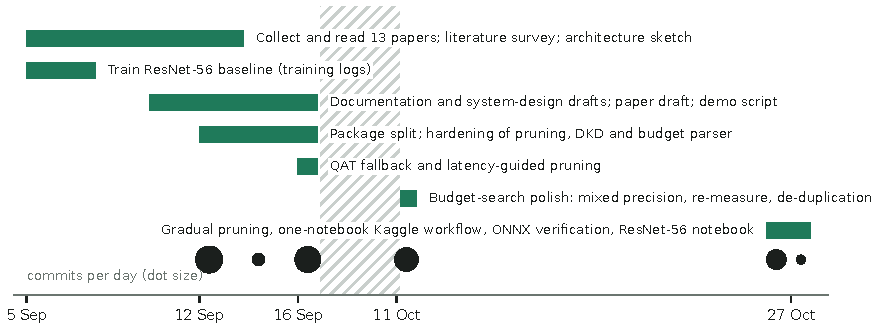
\includegraphics[width=\textwidth]{fig_timeline.pdf}
\caption{Project Timeline}
\label{fig:timeline}
\end{figure}


\chapter{Project Requirement Specification  }

\section{Hardware and Software Requirements}
\subsection{Hardware}
Two machines were used, with different roles; two of the runs in Section~\ref{sec:results} were also measured on an Intel Core i5-11320H laptop with fast INT8. The Apple laptop is the deployment-like target on which latency is judged; the Kaggle machine supplies a GPU for training and fine-tuning.

\begin{table}[!htbp]
\centering
\small
\begin{tabularx}{\textwidth}{@{}c l X X@{}}
\toprule
Sr. & Parameter & Local machine (final timing) & Kaggle notebook (training)\\
\midrule
1 & Processor & Apple M5, 10 logical cores (4 performance) & Intel Xeon @ 2.00 GHz, 4 logical cores\\
2 & INT8 support & Fast: i8mm, dotprod, fp16, bf16, neon & Slow: avx2, avx512f, f16c only\\
3 & Accelerator & None used & NVIDIA T4 GPU\\
4 & Role & Latency and ONNX verification & Training, fine-tuning, compression\\
\bottomrule
\end{tabularx}
\caption{Hardware Used}
\label{tab:hw}
\end{table}

\subsection{Software}

\begin{table}[!htbp]
\centering
\small
\begin{tabular}{@{}l l p{6.5cm}@{}}
\toprule
Component & Version / choice & Purpose\\
\midrule
Python & 3.14.7 (local) & Implementation language\\
PyTorch & 2.14.0 & Model definition, training, fine-tuning\\
Torch-Pruning & DepGraph pruner & Dependency-aware channel removal\\
ONNX Runtime & 1.29.0 & Quantization and all measurements\\
NumPy & 2.5.2 & Array operations, CPU feature flags\\
pytest & configured in \code{pyproject.toml} & 162 tests by default\\
Git and GitHub & -- & Version control and distribution\\
Kaggle Notebook & T4 GPU, internet on & Single end-to-end run environment\\
\bottomrule
\end{tabular}
\caption{Software Stack}
\label{tab:sw}
\end{table}





\section{Functional Requirement}
\begin{enumerate}
\item FR1: Train or load an FP32 classification baseline for CIFAR-10, a human-action-recognition dataset, or any one-folder-per-class image dataset.
\item FR2: Prune a model structurally by a requested ratio, in one or several steps, with per-layer alignment and shared ratios across residual groups.
\item FR3: Re-estimate batch-norm statistics and fine-tune with KD or DKD against the original model as teacher.
\item FR4: Quantize to INT8 or FP16 through ONNX Runtime, with an automatic choice gated by the host, and fall back to QAT when asked.
\item FR5: Rank layers by quantization sensitivity and use the ranking for exclusions and pruning ratios.
\item FR6: Accept a budget (latency, accuracy drop, minimum accuracy, size) and search for the cheapest configuration meeting it.
\item FR7: Benchmark every stage on the exported ONNX file and write \code{results.json}, an HTML report and the \code{.onnx} file.
\item FR8: Verify the compressed file against the original on real test images.
\end{enumerate}

\section{Non Functional Requirement }
\begin{itemize}
\item \textbf{Measurement integrity.} Latency uses one ONNX Runtime session configuration for every precision: one thread, batch size 1, 50 warm-up runs, 200 timed runs, median and 95th percentile reported. Accuracy is measured on the exported file.
\item \textbf{No leakage.} BN re-estimation and quantization calibration read only the training split.
\item \textbf{Reproducibility.} The train/test split of folder datasets is deterministic by sorted file name; random seeds are fixed for calibration subsets.
\item \textbf{Honest failure.} Unmet budgets return the best trade-off and say so. Operators without an INT8 kernel are counted in the report.
\item \textbf{Usability.} One command or one notebook run produces all outputs.
\item \textbf{Portability.} Pure Python, CPU inference, no vendor-specific runtime.
\end{itemize}
\section{Data Set Description/Database Schema }
\begin{description}
\item[CIFAR-10~\cite{krizhevsky2009}] 60,000 colour images of $32\times32$ pixels in 10 classes: 50,000 for training and 10,000 for testing. Used for ResNet-20, ResNet-56 and VGG-16-BN. Input shape for the toolkit: $1\times3\times32\times32$.
\item[Human Action Recognition (HAR)] A 15-class image dataset at $224\times224$ input, read through a loader that finds the data under the Kaggle input directory. The ResNet-18 baseline path is implemented; its Kaggle run was not completed within this project, so no HAR accuracy is claimed.
\item[Image folder] Any dataset with one sub-directory per class. A fixed 15\% of each class, taken from the end of the sorted file list, is held out as the test set.
\end{description}

\chapter{Proposed System}
\section{Overall System Architecture}
Fig.~\ref{fig:system} shows the whole system from what the user supplies to what it delivers. Three inputs go in: a trained FP32 checkpoint, a dataset with train, test and calibration views, and a request, which is either a fixed recipe (prune ratio, steps, fine-tune epochs, precision) or a budget string. The toolkit itself has five cooperating parts. An \emph{entry point} (command line, Python API or notebook) builds a \code{Pipeline}. The \emph{host probe} reads the CPU's instruction-set features and decides whether INT8 is allowed. The \emph{pipeline controller} checks the stage order and runs a pre-flight summary. The \emph{stages} transform the model in a fixed order. The \emph{search layer} sits beside them and, for a budget request, decides which stages to use. After every stage the \emph{measurement} component exports the model to ONNX and measures it in ONNX Runtime, and the \emph{reporting} component turns all measurements into the three outputs: the compressed \code{.onnx}, an HTML report and \code{results.json}. Finally the delivered file is re-measured on the target host and compared with the original.


\begin{figure}[H]
\centering
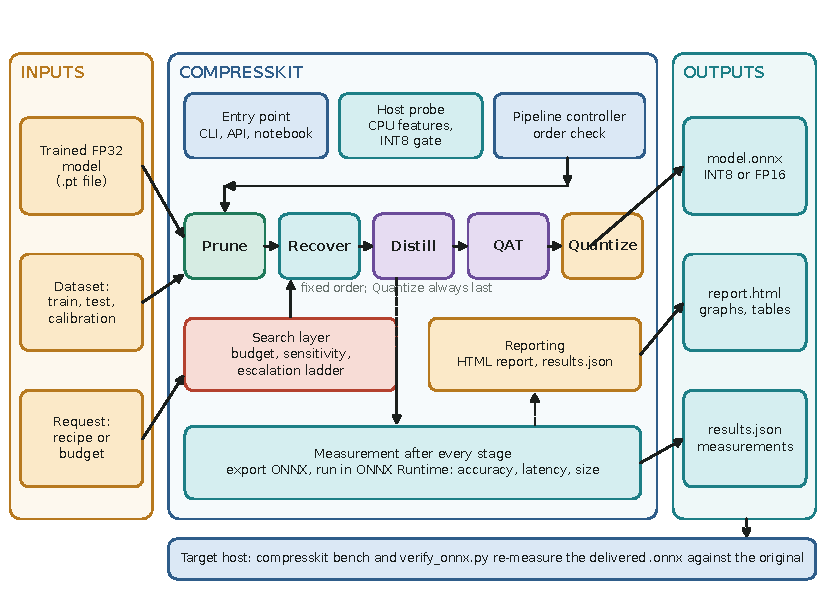
\includegraphics[width=\textwidth]{fig_system.pdf}
\caption{Overall System Architecture}
\label{fig:system}
\end{figure}
\section{Layered Architecture and Modules}
Seen as a code base, CompressKit is a small library with three entry points, four compression stages, an orchestration layer and a shared core (Fig.~\ref{fig:arch}). The core is cross-cutting: the host probe attaches the machine's capabilities to every measurement, the benchmark module produces the numbers all stages are judged by, and the export module writes ONNX.

\begin{figure}[H]
\centering
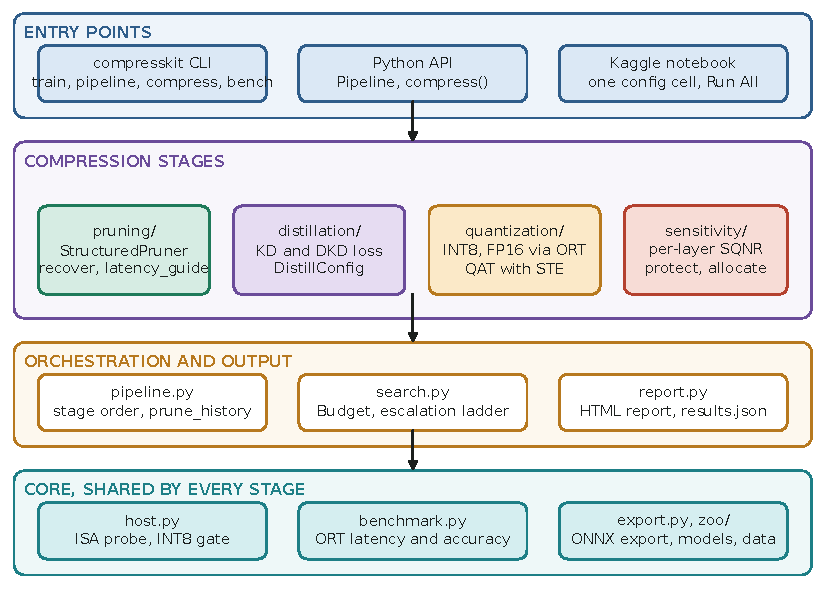
\includegraphics[width=0.66\textwidth]{fig_architecture.pdf}
\caption{Layered Architecture}
\label{fig:arch}
\end{figure}

\subsection{Modules}
\textbf{Host probe} (\code{core/host.py}). Reads the CPU's instruction-set features. INT8 is recommended only when at least one of AMX-INT8, AVX-512 VNNI, AVX-VNNI, I8MM or DotProd is present, because without a fused integer dot-product INT8 is routinely slower than FP32 while still producing a smaller file. Otherwise FP16 is the default and INT8 becomes an explicit, warned opt-in. The probe result is stored with each measurement.

\textbf{Structured pruner} (\code{pruning/prune.py}). Wraps Torch-Pruning's dependency graph~\cite{fang2023}. It never prunes the classifier, always works on a deep copy of the model, and adds three behaviours described next: per-layer SIMD alignment, shared ratios across residual groups, and gradual steps.

\textbf{Recovery} (\code{pruning/recover.py}). Resets batch-norm running statistics and recomputes them as a cumulative average over training batches, so the stale statistics of the old network are not applied to the new one.

\textbf{Distillation} (\code{distillation/distill.py}). KD and decoupled KD with the original, uncompressed model as teacher, so no second network has to be trained~\cite{chae2026}.

\textbf{Quantization} (\code{quantization/}). Static post-training quantization through ONNX Runtime with per-channel weights, calibrated on a subset of the training split, plus an operator-coverage audit; QAT with a straight-through estimator~\cite{bengio2013} as a fallback.

\textbf{Sensitivity} (\code{sensitivity/analysis.py}). Label-free per-layer ranking used for exclusions and non-uniform pruning ratios.

\textbf{Pipeline, search and report} (\code{pipeline.py}, \code{search.py}, \code{report.py}). Stage orchestration, the budget search, and the HTML and JSON output.

\section{The Compression Pipeline in Detail}
\subsection{Stage Model and Ordering Rule}
\begin{sloppypar}
The pipeline is a chainable builder: \code{Pipeline(model, calibration, test, train)} followed by calls such as \code{.prune(0.5, steps=3, fine\_tune\_epochs=2)}\allowbreak\code{.recover().quantize()} only \emph{records} the stages. Nothing runs until \code{run()}. Two copies of the model are made at construction. One is the untouched \emph{original}, which is both the accuracy reference and the distillation teacher, so it has to survive every in-place stage; the other is the working model.
\end{sloppypar}

One rule is enforced before any compute is spent: \code{quantize} must be the last stage, otherwise \code{run()} raises an error. Integer weights cannot be pruned structurally and cannot be trained further, so any stage placed after quantization would either fail or silently undo it~\cite{chae2026}. A \code{preflight()} call prints the host capabilities, parameter count, calibration size, the protected classifier layer and the planned stage list, and warns if quantize is not last.

\subsection{Stage by Stage}
Fig.~\ref{fig:pipedetail} gives the data path and Table~\ref{tab:stages} summarises what each stage takes, does and records.

\begin{figure}[H]
\centering
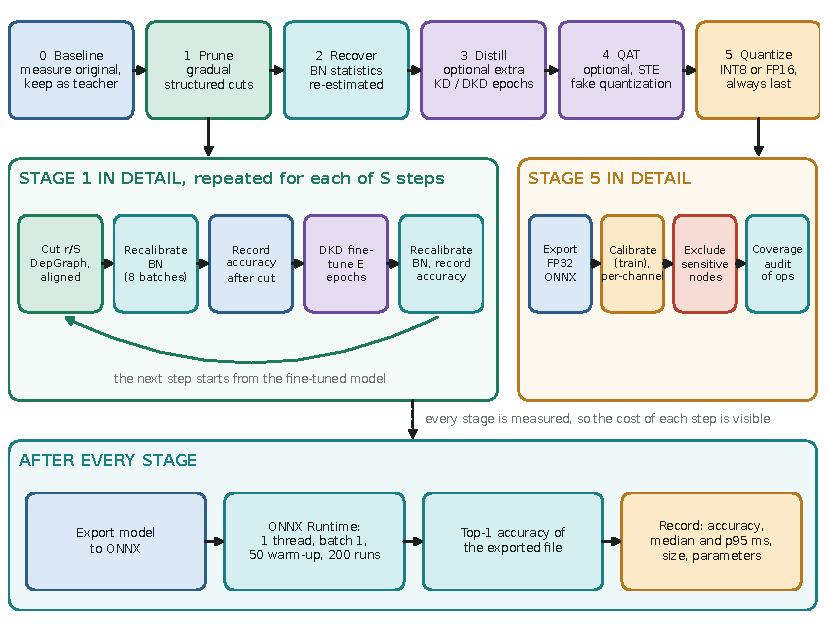
\includegraphics[width=\textwidth]{fig_pipeline_detail.pdf}
\caption{Detailed Compression Pipeline}
\label{fig:pipedetail}
\end{figure}

\begin{table}[!htbp]
\centering
\small
\setlength{\tabcolsep}{3pt}
\begin{tabularx}{\textwidth}{@{}l X X X@{}}
\toprule
Stage & What it does & Needs & Guard or record\\
\midrule
0 Baseline & Exports the original to ONNX and measures it & Test split & Teacher and reference for all later stages\\
1 Prune & $S$ cuts of $r/S$ of the channels, each followed by BN recalibration and DKD fine-tuning & Calibration and train loaders & Classifier never pruned; works on a deep copy; \code{prune\_history} rows\\
2 Recover & Resets BN running statistics and recomputes them as a cumulative average & Calibration loader (train split) & No labels, no back-propagation\\
3 Distill & Extra KD or DKD epochs against the original & Train loader & Error if no training data is given\\
4 QAT & Fake quantization with a straight-through estimator & Train loader & Fallback when post-training INT8 misses accuracy\\
5 Quantize & Exports FP32 ONNX, calibrates, writes INT8 or FP16 & Calibration loader, host probe & Sensitive layers excluded; operator coverage audited; must be last\\
\bottomrule
\end{tabularx}
\caption{Pipeline Stages}
\label{tab:stages}
\end{table}

\textbf{Pruning loop.} Each of the $S$ steps cuts a fraction of the channels, recalibrates the batch-norm statistics on eight calibration batches, records the accuracy right after the cut, fine-tunes for $E$ epochs with decoupled KD against the original, recalibrates again and records the accuracy after the fine-tune. Recalibrating between steps matters: the next importance ranking would otherwise be computed on a mis-normalised network. The last cut has no step after it, so it receives the same cut, fine-tune, recalibrate treatment explicitly. This is the code path where the defect described in Section~\ref{sec:defect} was found: the pruner works on its own deep copy, so the final fine-tune must act on the pruner's model and not on the caller's still-unpruned variable.

\textbf{Recover and distill.} Recovery needs no labels and costs a few forward passes. Distillation spends epochs of training and is used when fine-tuning inside the pruning loop is not enough.

\textbf{Quantize.} The working model is exported to an FP32 ONNX file; layer names from the sensitivity ranking are mapped to node names in \emph{that} exported graph; ONNX Runtime's static quantizer calibrates on the training subset with per-channel weight scales; and the result is audited for how many compute operators actually received an INT8 kernel. If the host probe reports no fused integer instructions, the default precision is FP16 and INT8 requires an explicit opt-in.

\textbf{Measurement.} After every stage the model is exported and measured under the same protocol. A stage's cost is therefore visible, and a stage that did not help (such as recovery after fine-tuning) shows as a flat step instead of being assumed useful.

\subsection{The Run Procedure}
\begin{algorithm}[H]
\caption{\code{Pipeline.run}}\label{alg:run}
\KwIn{ordered stages $T_1\dots T_n$, original model $M_0$, loaders}
\KwOut{list of measurements, prune history, warnings}
\lIf{quantize appears and is not last}{raise error}
baseline $\gets$ \textsc{Measure}($M_0$); $M \gets \mathrm{copy}(M_0)$\;
\For{$i \gets 1$ \KwTo $n$}{
  \Switch{kind of $T_i$}{
    \Case{prune}{ run Algorithm~\ref{alg:gradual} on $M$; $M \gets$ pruner's model }
    \Case{recover}{ recalibrate BN of $M$ on calibration batches }
    \Case{distill}{ distill $M$ from $M_0$ }
    \Case{qat}{ fake-quantize and fine-tune $M$ }
    \Case{quantize}{ export $M$; calibrate; write INT8 or FP16; audit coverage }
  }
  append \textsc{Measure}(result of $T_i$) to the list\;
}
\Return measurements, history, warnings\;
\end{algorithm}

\subsection{Why This Order}
Pruning first, because it changes the architecture and everything after must fit the smaller network. Batch-norm recalibration and distillation next, because they repair the accuracy lost by the cut while all weights are still float and trainable. Quantization last, because converting weights to integers is hard to reverse and blocks further training. The same order is used by the budget search, which differs only in \emph{how many} of these stages it applies.

\subsection{Two Ways to Drive the Pipeline}
In \emph{fixed-recipe mode} the user states the stages and their parameters, for example \code{compresskit pipeline --prune 0.5 --steps 3 --fine-tune-epochs 2}. In \emph{budget mode} the search layer builds one pipeline per ladder rung (Section~\ref{sec:budget}), runs it, compares the measurements with the budget and escalates only if the budget is unmet. Both modes call the same \code{Pipeline.run}, so every number in a report was produced by the same code path.

\section{Core Algorithms}
\subsection{Pruning: Residual Groups and Alignment}
In a residual network the output channels of a convolution may be summed with a shortcut, so several layers must keep exactly the same channel indices. Torch-Pruning exposes these as dependency groups. In ResNet-20, 12 groups tie two or more layers: three stage-wide groups of eight layers each, and nine groups that pair a convolution with its batch norm. If two layers in one group request different ratios the pruner would pick one arbitrarily. CompressKit resolves each group toward its most protective member, that is, the lowest requested ratio.


Channel counts are rounded to multiples of a SIMD-friendly alignment (8, 16 or 32). A single global alignment fails for narrow layers: Torch-Pruning floors the kept count to a multiple of the alignment, a layer whose width is under two alignment blocks floors to zero, the group is rejected as invalid, and the layer silently keeps every channel. The toolkit instead computes the nearest achievable aligned count per layer and halves the alignment only for the layer that needs it (Algorithm~\ref{alg:align}, Fig.~\ref{fig:align}).

\begin{algorithm}[H]
\caption{Per-layer aligned ratio (from \code{\_aligned\_ratio})}\label{alg:align}
\KwIn{layer width $w$, requested ratio $r$, alignment $a$}
\KwOut{effective ratio $r'$, alignment used $a'$}
$a' \gets a$\;
\While{$a' > 1$ \textbf{and} $\lfloor w / a' \rfloor < 2$}{$a' \gets \lfloor a'/2 \rfloor$}
\If{$a' \le 1$}{ $k \gets \max(1, \mathrm{round}(w(1-r)))$; \Return $(1-k/w,\ a')$ }
$n \gets \min\big(\lfloor w/a' \rfloor,\ \max(1,\ \mathrm{round}(w(1-r)/a'))\big)$\;
$k \gets n\,a'$; \Return $(1-k/w,\ a')$\;
\end{algorithm}

For example, a 64-channel layer at requested ratio 0.7 keeps 16 channels with alignment 16 (effective ratio 0.75) and 32 channels with alignment 32 (effective ratio 0.5): the result is the nearest multiple, not the floor. A 16-channel layer at ratio 0.5 keeps 8, and an 8-channel layer keeps 4 by relaxing the alignment to 4. These values come from a 180-case table generated by the real function, which is kept as a golden test of the alignment rule.

Figure~\ref{fig:align} plots the channels kept for layers of width 16 and 64 under alignments 8, 16 and 32. A narrow layer cannot satisfy a large alignment, so all curves coincide for the 16-channel layer.

\begin{figure}[H]
\centering
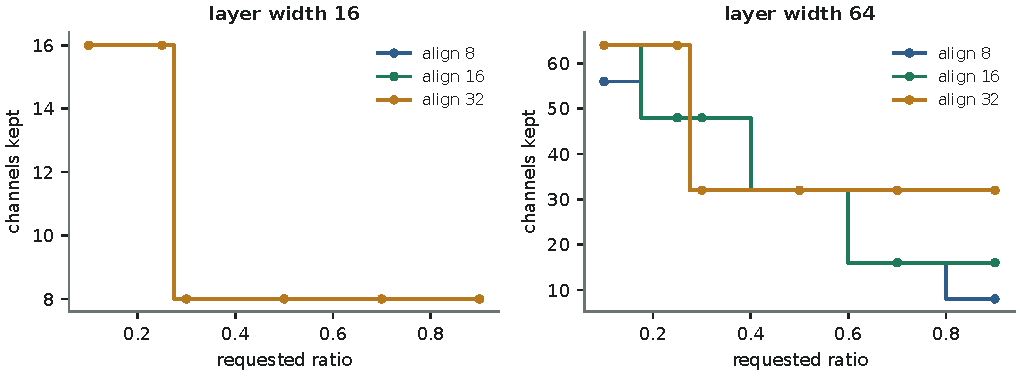
\includegraphics[width=\textwidth]{fig_align.pdf}
\caption{Channels Kept vs.\ Requested Pruning Ratio}
\label{fig:align}
\end{figure}

\subsection{Gradual Pruning with Fine-Tuning}
Instead of removing all channels at once, the pruner removes them in $S$ equal steps and fine-tunes after each (Algorithm~\ref{alg:gradual}). The motivation is that a smaller cut is easier to recover from~\cite{wang2025}; whether this beats one-shot pruning at an equal fine-tuning budget will be tested in Phase II. Every step is recorded as the accuracy right after the cut and right after the fine-tune.

\begin{algorithm}[H]
\caption{Gradual structured pruning with interleaved distillation}\label{alg:gradual}
\KwIn{trained model $M_0$ (teacher), ratio $r$, steps $S$, epochs per step $E$}
\KwOut{pruned model $M_S$, history of (acc. after cut, acc. after fine-tune)}
$P \gets \textsc{StructuredPruner}(\mathrm{copy}(M_0), r, S)$\;
\For{$s \gets 1$ \KwTo $S$}{
  $M \gets P.\mathrm{step}()$ \tcp*{remove $r/S$ of the way}
  record accuracy of $M$; recalibrate BN statistics on train batches\;
  \If{$E > 0$}{ fine-tune $M$ for $E$ epochs with DKD against $M_0$; record accuracy }
}
\Return $M$ (the pruner's own model, not the original)\;
\end{algorithm}

\subsection{Distillation Loss}
With student logits $z_s$, teacher logits $z_t$, temperature $T$ and target class $c$, decoupled KD~\cite{zhao2022} is
\begin{equation}
\mathcal{L}_{\mathrm{DKD}} = \alpha\, \mathrm{TCKD} + \beta\, \mathrm{NCKD},
\end{equation}
where TCKD is the KL divergence between the two-way distributions $(p_c,\,1-p_c)$ of teacher and student, and NCKD is the KL divergence between the teacher and student distributions over the non-target classes after masking the target before the softmax. Both terms are scaled by $T^2$. Defaults are $T=4$, $\alpha=1$ and $\beta=8$; plain KD uses $\alpha=0.3$. The final loss adds the cross-entropy on the labels. The target probability is clamped away from 0 and 1 so that a confident student cannot produce $\log 0$ and a NaN loss.

\subsection{Quantization and Sensitivity}
Weight quantization maps a tensor to 8-bit integers with a scale per output channel. The sensitivity of a layer is measured without labels: its weights alone are replaced by their INT8 quantize--dequantize round trip, and the signal-to-quantization-noise ratio at the output logits is computed,
\begin{equation}
\mathrm{SQNR}_\ell = 10\log_{10}\frac{\lVert y\rVert^2}{\lVert y-\hat{y}_\ell\rVert^2}\ \text{dB},
\end{equation}
where $\hat{y}_\ell$ are the logits with layer $\ell$ perturbed. For $L$ layers this takes $L+1$ forward passes. A low SQNR marks a layer that quantization hurts. The same ranking supplies the layers kept in FP32 and the layers that receive a smaller pruning ratio, which gives a non-uniform allocation without the reinforcement-learning search of~\cite{he2018}.

\subsection{Budget Search}\label{sec:budget}
A budget is a string such as \code{latency<0.45ms,accuracy\_drop<8\%}. \code{Budget.parse} turns it into limits on latency, accuracy drop, minimum accuracy and size. The search tries the cheapest rung first and moves on only if the budget is unmet (Fig.~\ref{fig:ladder}); borderline passes are re-measured at full fidelity before being trusted, and prune trials that resolve to an already measured architecture are skipped.

\begin{figure}[!htbp]
\centering
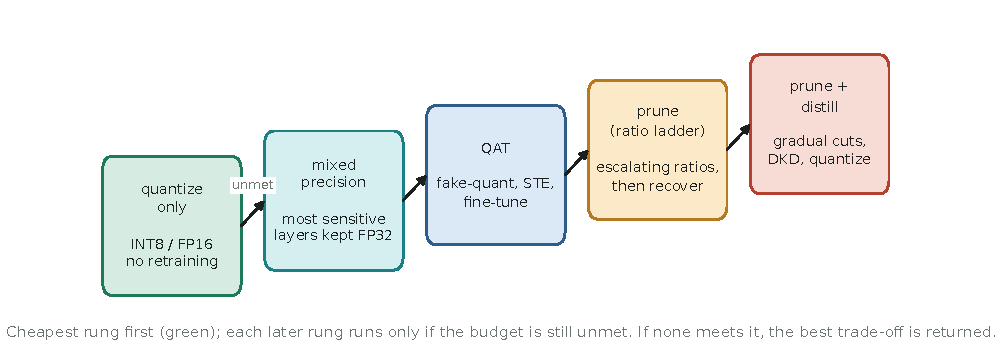
\includegraphics[width=\textwidth]{fig_ladder.pdf}
\caption{Budget Search Ladder}
\label{fig:ladder}
\end{figure}

\section{Data Flow Diagrams}
\subsection{DFD Level 0}
Level 0 shows the toolkit as a single process between the user, the dataset and the target runtime.
\begin{figure}[H]
\centering
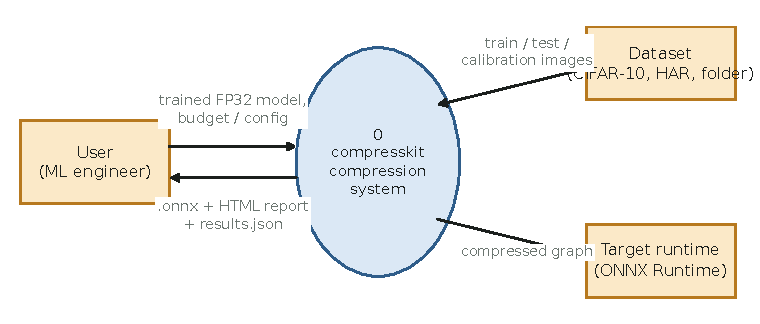
\includegraphics[width=0.62\textwidth]{fig_dfd0.pdf}
\caption{DFD Level 0}
\label{fig:dfd0}
\end{figure}

\subsection{DFD Level 1}
Level 1 breaks one compression run into its six processes.
\begin{figure}[H]
\centering
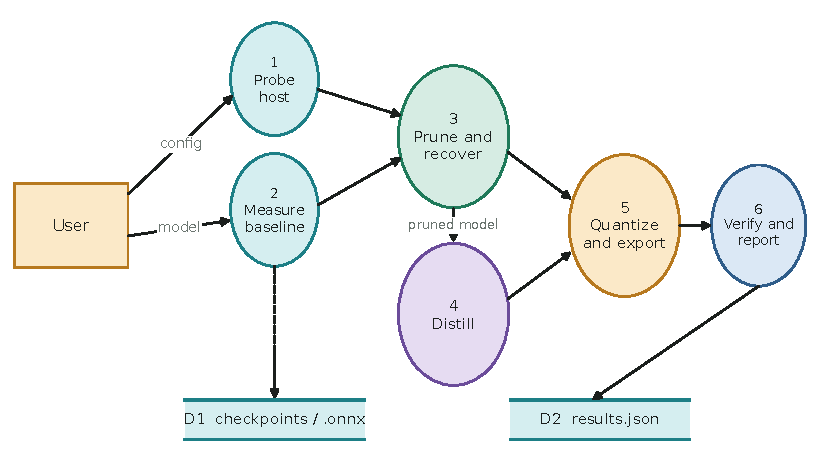
\includegraphics[width=\textwidth]{fig_dfd1.pdf}
\caption{DFD Level 1}
\label{fig:dfd1}
\end{figure}

\subsection{DFD Level 2}
Level 2 expands process 3 (prune and recover).
\begin{figure}[H]
\centering
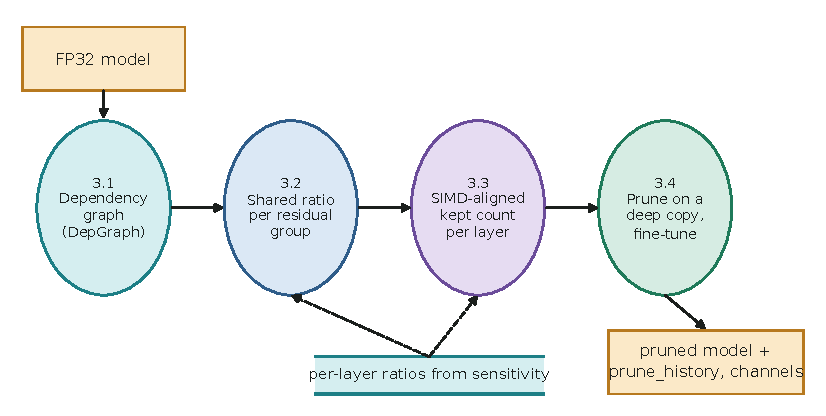
\includegraphics[width=\textwidth]{fig_dfd2.pdf}
\caption{DFD Level 2}
\label{fig:dfd2}
\end{figure}

\section{UML Diagrams}
\subsection{Use Case Diagram}
The target host CPU is a secondary actor, because latency and INT8 support are properties of that machine.
\begin{figure}[H]
\centering
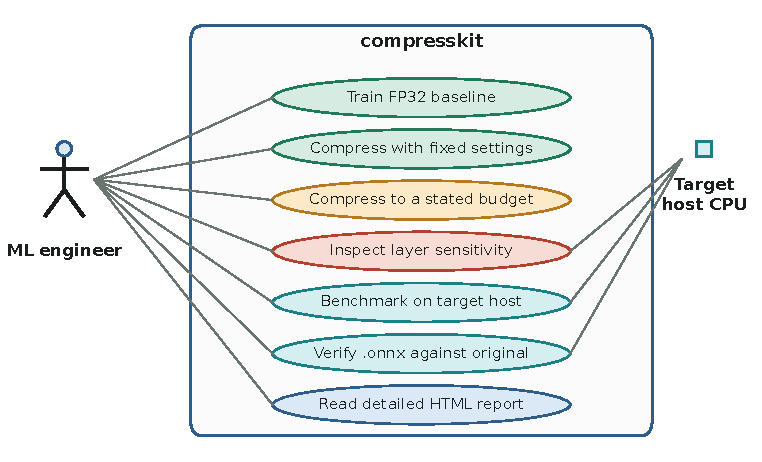
\includegraphics[width=0.6\textwidth]{fig_usecase.pdf}
\caption{Use Case Diagram}
\label{fig:usecase}
\end{figure}

\subsection{Sequence Diagram}
The sequence below follows one budget-driven \code{compress} run.
\begin{figure}[H]
\centering
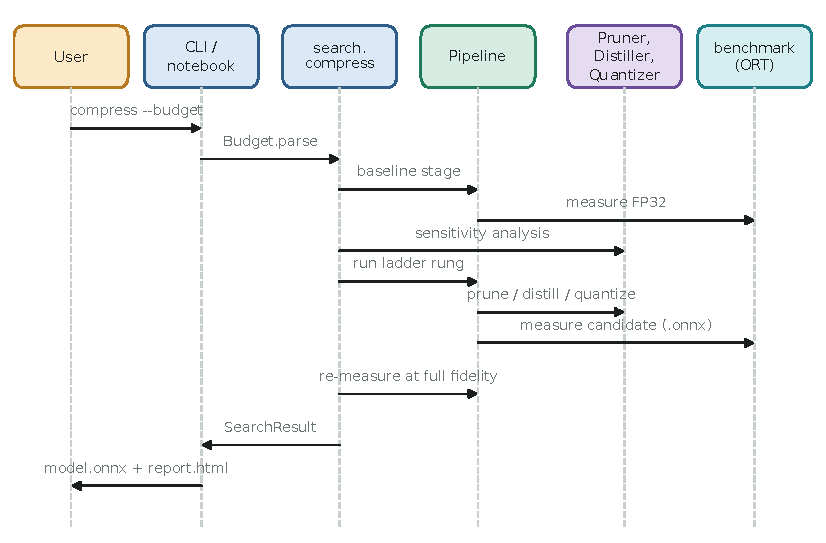
\includegraphics[width=\textwidth]{fig_sequence.pdf}
\caption{Sequence Diagram}
\label{fig:sequence}
\end{figure}

\subsection{Class Diagram}
The classes below are the main data carriers; each is a Python dataclass or a small class in the named module, and the field names are those in the source.
\begin{figure}[H]
\centering
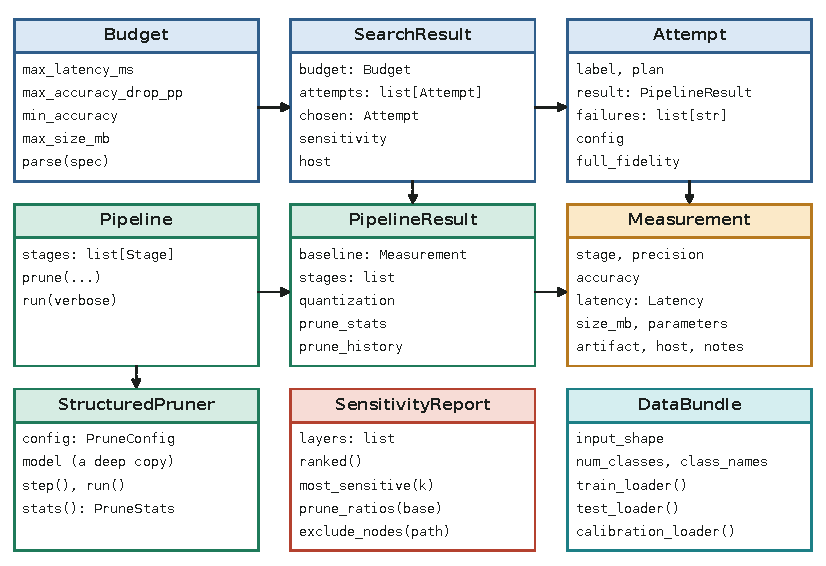
\includegraphics[width=\textwidth]{fig_classes.pdf}
\caption{Class Diagram}
\label{fig:classes}
\end{figure}

% =====================================================================
\chapter{System Implementation}
\section{Package Layout}
The package has 26 Python modules and 5,054 lines of source. The split into subpackages follows the stages, so a user can import the pruner without pulling in the quantizer. Project-specific code (the example networks and dataset loaders) lives in \code{zoo/} and is not part of the core API.

The largest modules are \code{search.py} (638 lines), \code{pruning/prune.py} (530), \code{report.py} (435), \code{pipeline.py} (420), \code{core/benchmark.py} (352) and \code{quantization/quantize.py} (338); the CLI is 329 lines and the example models, datasets and training code in \code{zoo/} about 700.

\section{Command-Line Interface}
The same flow is available from the command line. A complete run on CIFAR-10 is two commands:
\begin{lstlisting}[language=bash]
compresskit train --arch resnet20
compresskit pipeline --model checkpoints/resnet20_fp32.pt \
    --prune 0.5 --steps 3 --fine-tune-epochs 2 --loss dkd \
    --precision auto --report report.html
\end{lstlisting}
To compress to a requirement instead of a fixed recipe:
\begin{lstlisting}[language=bash]
compresskit compress --model checkpoints/resnet20_fp32.pt \
    --budget "latency<0.45ms,accuracy_drop<8%" --report report.html
\end{lstlisting}
Deployment latency on the target is re-measured with \code{compresskit bench model.onnx}, and the compressed file is compared with the original on real test images by the verification script \code{verify\_onnx.py}.

\section{Selected Code}
The per-layer alignment rule of Algorithm~\ref{alg:align}, as implemented:
\begin{lstlisting}[language=Python]
def _aligned_ratio(width, ratio, align):
    layer_align = align if align and align > 1 else 1
    while layer_align > 1 and width // layer_align < 2:
        layer_align //= 2
    if layer_align <= 1:
        kept = max(1, min(width, round(width * (1 - ratio))))
        return 1 - kept / width, layer_align
    desired_kept = width * (1 - ratio)
    max_blocks = width // layer_align
    n_blocks = min(max_blocks, max(1, round(desired_kept / layer_align)))
    kept = n_blocks * layer_align
    return 1 - kept / width, layer_align
\end{lstlisting}
The decoupled KD loss, including the numerical guard:
\begin{lstlisting}[language=Python]
def binary(prob):
    target_p = prob[target_mask].unsqueeze(1).clamp(min=1e-7, max=1.0 - 1e-7)
    return torch.cat([target_p, 1.0 - target_p], dim=1)

tckd = F.kl_div(binary(student_prob).log(), binary(teacher_prob),
                reduction="batchmean") * (temperature ** 2)
masked_student = student_logits / temperature - 1000.0 * target_mask
masked_teacher = teacher_logits / temperature - 1000.0 * target_mask
# nckd: KL between the renormalised non-target distributions, scaled by T**2
return alpha * tckd + beta * nckd
\end{lstlisting}

The ordering rule is checked before any compute is spent (\code{pipeline.py}):
\begin{lstlisting}[language=Python]
def run(self, verbose: bool = True) -> PipelineResult:
    kinds = [stage.kind for stage in self.stages]
    if "quantize" in kinds and kinds.index("quantize") != len(kinds) - 1:
        raise ValueError(
            "quantize must be the last stage - it changes weight dtype, "
            "which breaks structural pruning and blocks further fine-tuning"
        )
\end{lstlisting}
INT8 is chosen only when the host has fused integer kernels (\code{core/host.py}):
\begin{lstlisting}[language=Python]
@property
def int8_speed(self) -> str:
    """'fast' | 'slow' | 'unknown' - whether INT8 has a fused kernel path."""
    if self.int8_features:
        return "fast"
    if not self.features:
        return "unknown"
    return "slow"

@property
def recommended_precision(self) -> str:
    """Default precision for this host. INT8 only where it will pay off."""
    return "int8" if self.int8_speed == "fast" else "fp16"
\end{lstlisting}

\section{One-Notebook Workflow}
The project fixed one working environment. Code lives on GitHub; one Kaggle notebook (\code{kaggle/compresskit\_end\_to\_end.ipynb}) does setup, data, training, compression, ONNX evaluation and report generation under \emph{Run All}, driven by one configuration cell (model, mode manual or budget, prune ratio, steps, fine-tune epochs, loss, precision). Models are not copied between machines while the work runs; the output folder is downloaded once at the end and the final latency check runs on the local machine. Because the Kaggle CPU has no fast INT8, the notebook forces INT8 when asked and the report states that its latency is not the target's.

\section{A Defect Found by Verification}\label{sec:defect}
The first end-to-end ResNet-20 run printed 88\% accuracy in its log, but loading the exported \code{.onnx} and testing it on real images gave 47\%. The cause was in the pipeline: the pruner operates on a deep copy of the model, and the final fine-tune step was applied to the original, unpruned model, while the exported graph came from the pruner's copy. The fix is one line, fine-tuning \code{pruner.model} instead of the caller's variable, and a regression test (\code{test\_every\_fine\_tune\_step\_acts\_on\_the\_pruned\_model}) was written first, shown to fail on the old code and to pass after the change. This is why accuracy is measured on the exported file and not on the in-memory model.

\section{Compression Results}\label{sec:results}
The toolkit was run end to end on five model configurations: three architectures on CIFAR-10 and one on the Human Action Recognition (HAR) dataset, with ResNet-20 compressed under two different schedules. Table~\ref{tab:models} lists what was applied to each model and Table~\ref{tab:results} gives the measured results. The hosts are an Apple M5, an Intel Core i5-11320H and the Kaggle CPU (Intel Xeon). Every latency is the median of 200 runs at batch size 1 on one thread after 50 warm-up runs, and every accuracy is the top-1 accuracy of the exported ONNX file on the held-out test split.

\begin{table}[H]
\centering
\small
\begin{tabularx}{\textwidth}{@{}l l >{\raggedright\arraybackslash}X l r@{}}
\toprule
\textbf{Model} & \textbf{Dataset} & \textbf{Compression applied} & \textbf{Measured on} & \textbf{Parameters}\\
\midrule
ResNet-20 & CIFAR-10 & 50\% pruning in 3 steps (2 DKD epochs each), INT8 & Apple M5 & 272K $\to$ 69K\\
ResNet-20 & CIFAR-10 & 50\% pruning (25\% in last stage) in 5 steps, INT8 & Intel i5 & 272K $\to$ 129K\\
ResNet-56 & CIFAR-10 & 50\% pruning (25\% in last stage) in 5 steps, INT8 & Intel i5 & 856K $\to$ 414K\\
VGG-16-BN & CIFAR-10 & 50\% pruning in 5 steps (5 DKD epochs each), INT8 & Kaggle CPU & 14.72M $\to$ 3.68M\\
ResNet-18 & HAR & INT8 only (no pruning) & Apple M5 & 11.19M (same)\\
\bottomrule
\end{tabularx}
\caption{Compressed Models}
\label{tab:models}
\end{table}

\begin{table}[H]
\centering
\small
\setlength{\tabcolsep}{3.5pt}
\begin{tabular}{@{}l c c c c c@{}}
\toprule
\textbf{Model (host)} & \textbf{Top-1 (\%)} & \textbf{Latency (ms)} & \textbf{Speed-up} & \textbf{Size (MB)} & \textbf{Smaller}\\
\midrule
ResNet-20 (M5)     & 91.54 $\to$ 84.00 & 1.452 $\to$ 0.460  & 3.16$\times$ & 1.05 $\to$ 0.11  & 9.11$\times$ \\
ResNet-20 (i5)     & 91.54 $\to$ 87.11 & 0.612 $\to$ 0.313  & 1.95$\times$ & 1.05 $\to$ 0.17  & 6.01$\times$ \\
ResNet-56 (i5)     & 93.18 $\to$ 90.50 & 1.892 $\to$ 0.842  & 2.25$\times$ & 3.28 $\to$ 0.53  & 6.20$\times$ \\
VGG-16-BN (Kaggle) & 93.20 $\to$ 90.18 & 9.042 $\to$ 1.133  & 7.98$\times$ & 56.16 $\to$ 3.57 & 15.72$\times$\\
ResNet-18 (M5)     & 75.50 $\to$ 74.66 & 15.772 $\to$ 8.510 & 1.85$\times$ & 42.66 $\to$ 10.79 & 3.96$\times$\\
\bottomrule
\end{tabular}
\caption{Compression Results (Baseline $\to$ Compressed)}
\label{tab:results}
\end{table}

All five runs produced a smaller and faster model, with size reductions from 3.96$\times$ to 15.72$\times$ and speed-ups from 1.85$\times$ to 7.98$\times$. The two ResNet-20 runs show the trade-off a schedule controls: cutting 75\% of the parameters in three steps gave the larger speed-up (3.16$\times$) but lost 7.54 points of accuracy, while the gentler five-step schedule lost 4.43 points. ResNet-18 on HAR was quantized without pruning, so its parameter count is unchanged and its 1.85$\times$ speed-up comes from INT8 alone. The VGG-16-BN figures were typed in from the printed log of the Kaggle run, and its latency was measured on the Kaggle CPU, which has no fast INT8 path; most of that speed-up therefore comes from pruning rather than quantization.

 %
  %


     
\chapter{Conclusion and Future Scope}
Section~\ref{sec:results} reports the measured results of five compression runs. The outcomes stated below go beyond those runs and are projections from the evaluation protocol and the cited literature.

\section{Measured Baseline}
ResNet-56 achieves an accuracy of 93.18\% on the held-out 10,000-image CIFAR-10 test set after 60 epochs of training with warm-up and cosine learning-rate scheduling.

\section{Expected Compression Results}
The sweep evaluates pruning ratios $r \in \{0.0,\ 0.3,\ 0.5,\ 0.7\}$ at FP32 and INT8 precision, with optional distillation recovery. Accuracy is expected to decline as pruning increases, while distillation should recover part of the loss.

At low pruning ratios, macro precision and recall should broadly track Top-1 accuracy. At higher ratios, per-class degradation is expected to become non-uniform, particularly for visually similar pairs such as cat/dog and automobile/truck. The full confusion matrix is accumulated during the same evaluation pass, and partial search evaluations are flagged and re-measured on the complete test set before reporting.

\section{Expected Effect of the Contributed Mechanisms}
Precision gating should expose hosts where INT8 is smaller but not faster: without fused integer kernels, a size reduction of about $4\times$ with unchanged or worse latency is expected. Protecting the two lowest-SQNR layers is expected to improve accuracy relative to uniform pruning at matched compression. Operator coverage below one should correspond to the remaining floating-point operators and explain cases where size decreases without an improvement in latency.

\section{Threats to Validity}
Current validation covers the evaluated architectures; grouped or depth-wise convolutions, such as those in MobileNet, require separate testing. Alignment protection applies to local pruning only, SQNR is a weight-only proxy, quantization exclusions are not automatic in the search, and latency is host-specific.

% \bibliographystyle{plain}

%\bibliographystyle{ieeetr}
%\bibliography{biblo}

% ------------------------------------------------------------ appendix (before references)
\appendix
\chapter{Paper Plagiarism Report}
This appendix contains the screenshot of the Turnitin plagiarism report of the project paper (Submission ID: trn:oid:::9832:158852096). Figure~\ref{fig:turnitin} shows the Integrity Overview, which records an overall similarity of 6\%.

\begin{figure}[H]
\centering
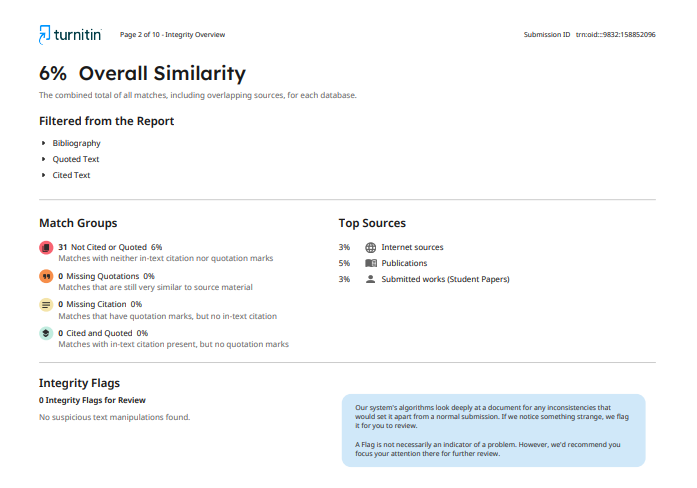
\includegraphics[width=\linewidth]{fig_plag_report_crop.png}
\caption{Turnitin Integrity Overview}
\label{fig:turnitin}
\end{figure}

% ------------------------------------------------------------ references
\renewcommand{\bibname}{References}
\begin{thebibliography}{99}
\bibitem{wang2025} Z. Wang, L. Shi, Z. Mei, X. Zhao, Z. Wang, and J. Li, ``Iterative knowledge distillation and pruning for model compression in unsupervised domain adaptation,'' Pattern Recognition, vol. 164, art. 111512, 2025, doi: 10.1016/j.patcog.2025.111512.

\bibitem{hinton2015} G. Hinton, O. Vinyals, and J. Dean, ``Distilling the Knowledge in a Neural Network,'' in NIPS Deep Learning and Representation Learning Workshop, 2015, arXiv:1503.02531.

\bibitem{chae2026} W. Chae and K. Seo, ``Pipeline of Pruning, Knowledge Distillation, and Quantization for Model Compression,'' Journal of Electrical Engineering \& Technology, vol. 21, pp. 2099–2105, 2026, doi: 10.1007/s42835-025-02541-7.

\bibitem{abdelsalam2025} R. Abdel-Salam, A. H. Abdel-Gawad, and A. G. Wassal, ``VLCQ: Post-training quantization for deep neural networks using variable length coding,'' Future Generation Computer Systems, vol. 166, art. 107654, 2025, doi: 10.1016/j.future.2024.107654.

\bibitem{khan2025} N. A. Khan and A. M. S. Rafat, ``Optimizing Deep Learning Models for Resource-Constrained Environments With Cluster-Quantized Knowledge Distillation,'' Engineering Reports, vol. 7, art. e70187, 2025, doi: 10.1002/eng2.70187.

\bibitem{he2018} Y. He, J. Lin, Z. Liu, H. Wang, L.-J. Li, and S. Han, ``AMC: AutoML for Model Compression and Acceleration on Mobile Devices,'' in Proc. European Conference on Computer Vision (ECCV), 2018.

\bibitem{chen2021} W. Chen, H. Qiu, J. Zhuang, C. Zhang, Y. Hu, Q. Lu, T. Wang, Y. Shi, M. Huang, and X. Xu, ``Quantization of Deep Neural Networks for Accurate Edge Computing,'' ACM Journal on Emerging Technologies in Computing Systems, vol. 17, no. 4, art. 54, 2021, doi: 10.1145/3451211.

\bibitem{fang2026} X. Fang, L. Chen, H. Yin, X. Chen, and W. Wang, ``Communication Efficient Federated Learning With Quantization-Aware Training Design,'' IEEE Transactions on Machine Learning in Communications and Networking, vol. 4, pp. 45–59, 2026, doi: 10.1109/TMLCN.2025.3635050.

\bibitem{he2016} K. He, X. Zhang, S. Ren, and J. Sun, ``Deep Residual Learning for Image Recognition,'' in Proc. IEEE Conference on Computer Vision and Pattern Recognition (CVPR), 2016, pp. 770--778.

\bibitem{simonyan2015} K. Simonyan and A. Zisserman, ``Very Deep Convolutional Networks for Large-Scale Image Recognition,'' in Proc. International Conference on Learning Representations (ICLR), 2015.

\bibitem{jacob2018} B. Jacob, S. Kligys, B. Chen, M. Zhu, M. Tang, A. Howard, H. Adam, and D. Kalenichenko, ``Quantization and Training of Neural Networks for Efficient Integer-Arithmetic-Only Inference,'' in Proc. IEEE Conference on Computer Vision and Pattern Recognition (CVPR), 2018, pp. 2704--2713.

\bibitem{zhao2022} B. Zhao, Q. Cui, R. Song, Y. Qiu, and J. Liang, ``Decoupled Knowledge Distillation,'' in Proc. IEEE/CVF Conference on Computer Vision and Pattern Recognition (CVPR), 2022, pp. 11953--11962.

\bibitem{xu2024} L. Xu, J. Ren, Z. Huang, W. Zheng, and Y. Chen, ``Improving Knowledge Distillation via Head and Tail Categories,'' IEEE Transactions on Circuits and Systems for Video Technology, vol. 34, no. 5, pp. 3465–3478, 2024, doi: 10.1109/TCSVT.2023.3325814.

\bibitem{zhou2026} M. Zhou, R. Mao, S. Sripada, and X. Li, ``AEMC: Aggregator-efficient model compression for streamlining LLMs,'' Neurocomputing, vol. 672, art. 132779, 2026, doi: 10.1016/j.neucom.2026.132779.

\bibitem{chen2020} Y. Chen, C. Li, L. Gong, X. Wen, Y. Zhang, and W. Shi, ``A deep neural network compression algorithm based on knowledge transfer for edge devices,'' Computer Communications, vol. 163, pp. 186–194, 2020, doi: 10.1016/j.comcom.2020.09.016.

\bibitem{krizhevsky2009} A. Krizhevsky, ``Learning Multiple Layers of Features from Tiny Images,'' Technical Report, University of Toronto, 2009.

\bibitem{fang2023} G. Fang, X. Ma, M. Song, M. B. Mi, and X. Wang, ``DepGraph: Towards Any Structural Pruning,'' in Proc. IEEE/CVF Conference on Computer Vision and Pattern Recognition (CVPR), 2023, pp. 16091--16101.

\bibitem{bengio2013} Y. Bengio, N. L\'eonard, and A. Courville, ``Estimating or Propagating Gradients Through Stochastic Neurons for Conditional Computation,'' arXiv:1308.3432, 2013.
\end{thebibliography}

\end{document}
